\documentclass[tikz]{standalone}
\usepackage{pgfplots}
\pgfplotsset{compat=1.15}
\usepackage{mathrsfs}
\usetikzlibrary{arrows,calc}
\usepackage{tkz-euclide}
\pagestyle{empty}

\definecolor{AngleClr}{rgb}{0,0.39215686274509803,0}
\definecolor{ShapeClr}{rgb}{0.6,0.2,0}
\definecolor{BlueSqr}{RGB}{5,81,163}
\definecolor{RedSqr}{RGB}{0, 156, 0}

\begin{document}

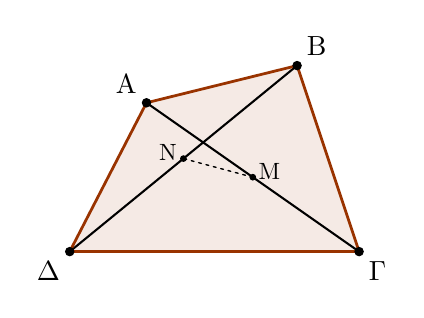
\begin{tikzpicture}[scale=.75]
\tkzSetUpLine[line width=1pt,color=black]
\tkzSetUpPoint[fill=black]

\tkzDefPoints{0/0/D,4.9/0/C,1.3/2.52/A,3.85/3.15/B}

\tkzFillPolygon[fill=ShapeClr,fill opacity=0.1](A,B,C,D)


\tkzDefMidPoint(A,C) \tkzGetPoint{M}
\tkzDefMidPoint(B,D) \tkzGetPoint{N}

\tkzDrawSegments[line width=0.75pt,color=black](A,C B,D)

\tkzDrawPolygon[color=ShapeClr](A,B,C,D)
\tkzDrawPoints[size=3](A,B,C,D)
\tkzDrawPoints[size=2](M,N)
\tkzLabelPoint[above left](A){$\rm A$}
\tkzLabelPoint[above right](B){$\rm B$}
\tkzLabelPoint[below right](C){$\rm \Gamma$}
\tkzLabelPoint[below left](D){$\rm \Delta$}
\node[scale=0.85,yshift=0.09cm, xshift=0.25cm] at (M) {$\rm M$};
\node[scale=0.85,yshift=0.09cm, xshift=-0.23cm] at (N) {$\rm N$};

\tkzDrawSegment[line width=0.5pt,color=black,dashed,dash pattern=on 1pt off 1.75pt](M,N)

\end{tikzpicture}

\end{document}
